% Figure 5 — Hostel-Administrator Activities (dark-header boxes, like the reference)
\documentclass[border=12pt]{standalone}
\usepackage{tikz}
\usepackage[table]{xcolor}
\usetikzlibrary{arrows.meta, fit}
\begin{document}
\small
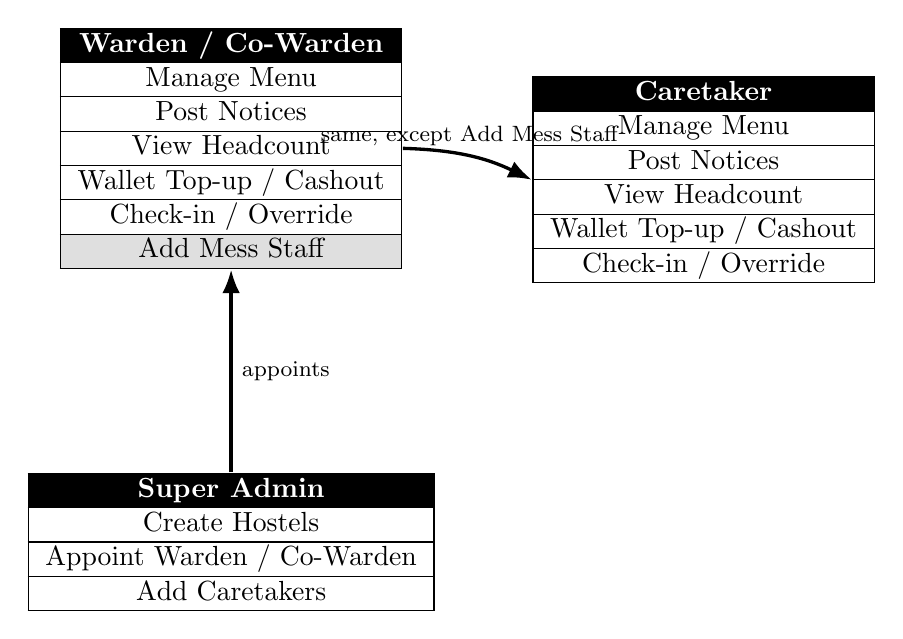
\begin{tikzpicture}[
    flow/.style={-{Latex[length=3mm]}, very thick},
  ]

  % ---- Warden / Co-Warden panel ----
  \node[inner sep=0pt] (warden) at (0,0) {%
    \begin{tabular}{|c|}
      \hline \rowcolor{black}\color{white}\bfseries Warden / Co-Warden \\ \hline
      Manage Menu \\ \hline Post Notices \\ \hline View Headcount \\ \hline
      Wallet Top-up / Cashout \\ \hline Check-in / Override \\ \hline
      \cellcolor{gray!25}Add Mess Staff \\ \hline
    \end{tabular}};

  % ---- Caretaker panel ----
  \node[inner sep=0pt] (care) at (6,-0.4) {%
    \begin{tabular}{|c|}
      \hline \rowcolor{black}\color{white}\bfseries Caretaker \\ \hline
      Manage Menu \\ \hline Post Notices \\ \hline View Headcount \\ \hline
      Wallet Top-up / Cashout \\ \hline Check-in / Override \\ \hline
    \end{tabular}};

  % Caretaker = Warden minus "Add Mess Staff"
  \draw[flow] (warden.east) to[bend left=12]
      node[above, font=\footnotesize]{same, except Add Mess Staff} (care.west);

  % ---- Super Admin appoints the hostel admins ----
  \node[inner sep=0pt] (super) at (0,-5) {%
    \begin{tabular}{|c|}
      \hline \rowcolor{black}\color{white}\bfseries Super Admin \\ \hline
      Create Hostels \\ \hline Appoint Warden / Co-Warden \\ \hline
      Add Caretakers \\ \hline
    \end{tabular}};
  \draw[flow] (super.north) -- node[right, font=\footnotesize]{appoints} (warden.south);

\end{tikzpicture}
\end{document}
